\documentclass[]{beamer}
\usetheme{KUL}
\usepackage{multirow}
\usepackage{multicol}
\usepackage{tikz}
\usepackage{ulem}
\usepackage{siunitx}
\newcommand\itemS{\item[\textbf{\S}]}
\definecolor{darkgreen}{rgb}{0,0.598,0.199}
\usepackage{times} % set font on times new roman
\usepackage{eurosym} % package for Euro sign
\usepackage{lineno}   % package for line numbering
\usepackage{hyperref} % this is for url links
\usepackage{subcaption}  % this package enables one to put several figures next to each other
\usepackage{textcomp}
\usepackage{setspace}
\usepackage{gensymb}

%----------------------------------
% Fill in the essential Information
%----------------------------------

\title[Individualizaci\'on de filamentos mediante optimizaci\'on]{Propuesta de Tesis: Individualizaci\'on de filamentos en una red mediante optimizaci\'on}
%\subtitle{\ldots a subtitle}
\author[L.\ Pizarro]{Leonardo Pizarro} % between [] is short name, between {} is long name
\date{\today} % Here you can also just type something, e.g. October 10, 2017
\institute[DCC - FCFM - UChile]{Facultad de Ciencias F\'isicas y Matem\'aticas\\ Departmento de Ciencias de la Computaci\'on \\ Universidad de Chile}

%----------------------------------
% ACTUAL PRESENTATION STARTS HERE
%----------------------------------

\begin{document}

% TITEL PAGE	
	{
		\setbeamertemplate{headline}{} %define local, empty header for title page
		\setbeamertemplate{footline}{} %define local, empty footer for title page
		\maketitle
	}
	\addtocounter{framenumber}{-1} % We don't count the title page

\begin{frame}
\frametitle{Contenidos} 
\tableofcontents
\end{frame}

% FRAME 1 
\section{Contexto}
\begin{frame}{}
% encontramos filamentos en todos lados (poner imagenes)
% que entendemos por filamento: estructura alargada no totalmente recta ...
% formas actuales de analisis: enfoques, 
\begin{itemize}
    \item 
    
\end{itemize}
\begin{kulblock}{Landslide}
    A landslide is the downhill movement of soil mass
\end{kulblock}
\end{frame}

% FRAME 2
\begin{frame}{}
    \begin{columns}[t]
        \column{.5\textwidth}
        \centering
        
\includegraphics[height=3.5cm]{Pictures/define-weighted-4.png}
        \captionof{figure}{Representaci\'on simplificada de una red con cruces y sobreposici\'on de filamentos en una imagen de microscop\'ia}

        \column{.5\textwidth}
        \centering
        
\includegraphics[height=3.5cm]{Pictures/define-weighted-4-bw-invert.png}
        \captionof{figure}{Preprocesamiento de la imagen mediante segmentaci\'on para la extracci\'on de la red}
    \end{columns}
\end{frame}


\begin{frame}{}
    \begin{columns}[t]
        \column{.5\textwidth}
        \centering
        
\includegraphics[height=3.5cm]{Pictures/skel_in_segment.png}
        \captionof{figure}{Esqueletonizaci\'on representativa de la red sobre la imagen de }
        
        \column{.5\textwidth}
        \centering
        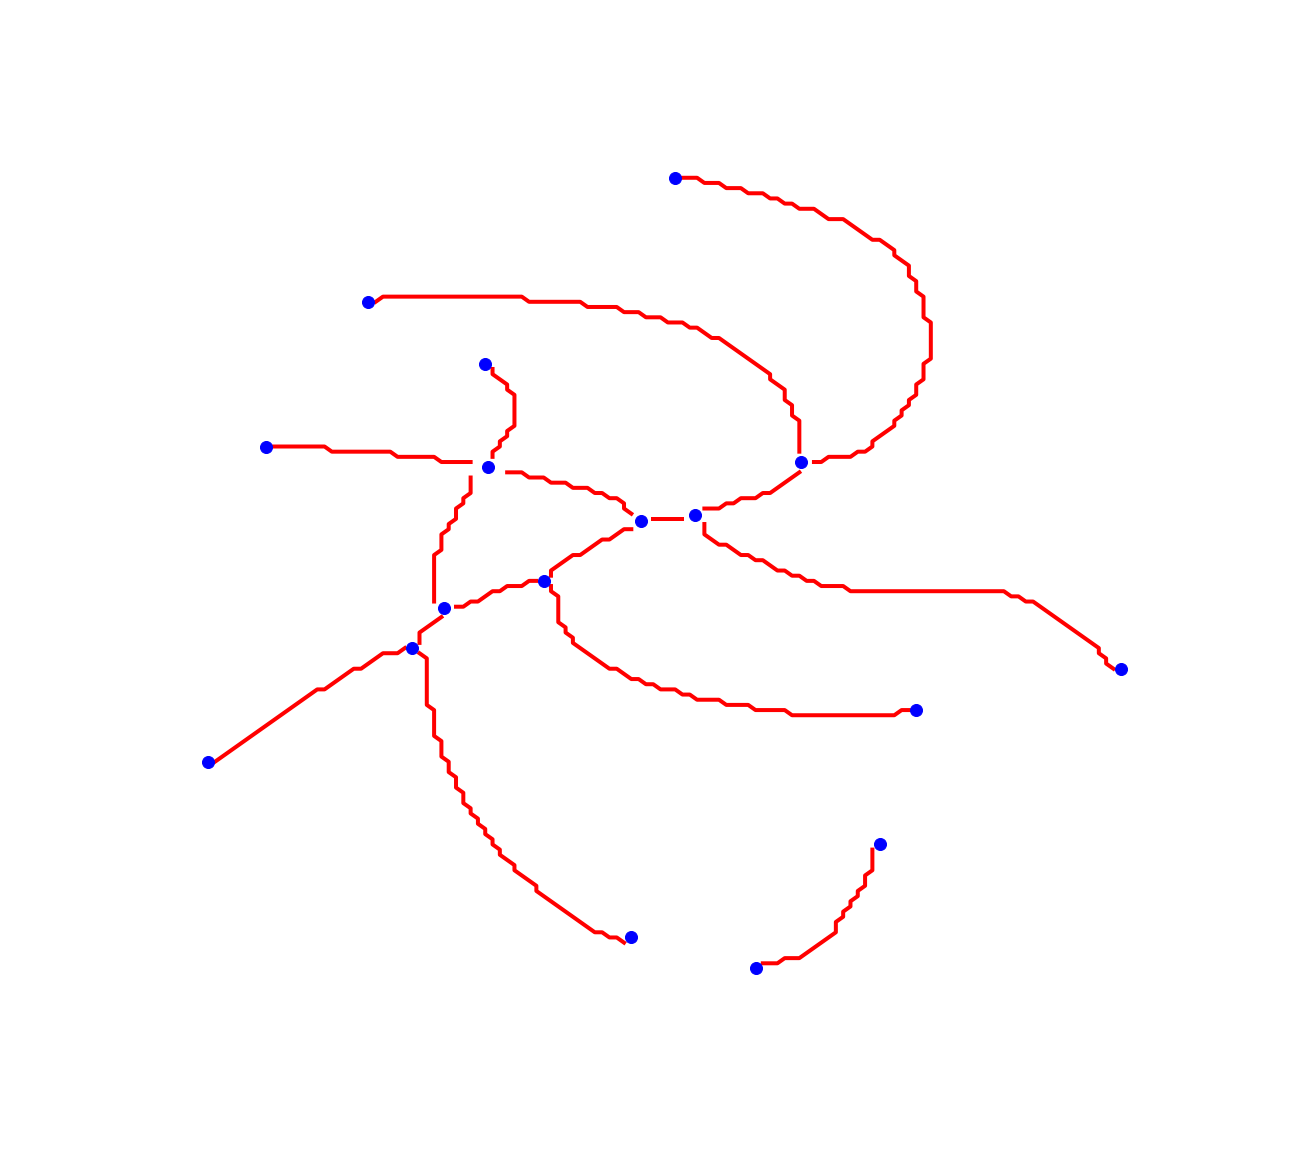
\includegraphics[height=3.5cm]{Pictures/graph_of_skel_no_axis.png}
        \captionof{figure}{Procedimiento para obtener un grafo que representa la red, a partir del procesamiento de una imagen de microscop\'ia, utilizando segmentaci\'on y esqueletonizaci\'on}
    \end{columns}
\end{frame}


\section{Antecedentes}

\begin{frame}{}
    \begin{columns}[t]
        \column{.5\textwidth}
        \centering
        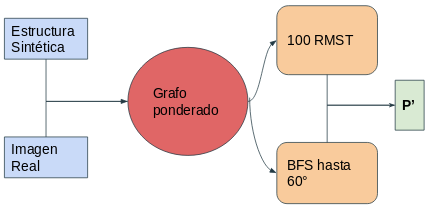
\includegraphics[width=\textwidth]{Pictures/flujoDefine.png}
        \captionof{figure}{Entrada de datos y elecci\'on de subconjunto de caminos {\bf P'} en DeFine}
        
        \column{.5\textwidth}
        \centering
        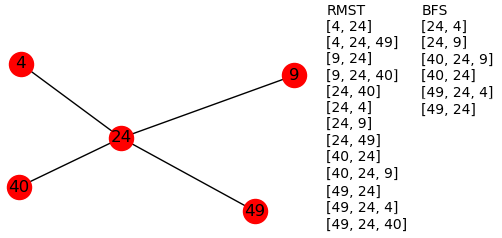
\includegraphics[width=\textwidth]{Pictures/BFSvsRMSTpaths.png}
        \captionof{figure}{Subconjunto {\bf P'} para el grafo de 5 nodos a la izquierda, utilizando la opci\'on de 100 {\it RMST} o heur\'istica de {\it BFS} que corta el camino al encontrar un \'angulo de deflexi\'on mayor a 60\degree entre aristas adyacentes}
    \end{columns}
\end{frame}

% FRAME 3
\begin{frame}{}
\centering
\begin{tabular}{|c|c|}
    \hline
     \bf X & \bf Y \\ \hline
     x & y \\ \hline 
\end{tabular}
\end{frame}

\begin{frame}{}
    \begin{columns}[t]
        \column{.5\textwidth}
        \centering
        
\includegraphics[width=\textwidth]{Pictures/define-weighted-4-expected2.png}
        \captionof{figure}{Visualizaci\'on de un resultado posible de individualizaci\'on, limitando los filamentos identificados a estructuras simples}
        
        \column{.5\textwidth}
        \centering
        
\includegraphics[width=\textwidth]{Pictures/define-weighted-4-expected1.png}
        \captionof{figure}{Visualizaci\'on de otro resultado posible de individualizaci\'on, permitiendo filamentos m\'as complejos}
    \end{columns}
\end{frame}

\begin{frame}{Visualizaci\'on de Microt\'ubulos}
    \begin{columns}[t]
        \column{.5\textwidth}
        \centering
        \includegraphics[width=\textwidth]{Pictures/ArabidopsisMT.png}
        % \captionof{figure}{}
        
        \column{.5\textwidth}
        \centering
        \includegraphics[width=\textwidth]{Pictures/ArabidopsisMT-Zmax.png}
        %  \captionof{figure}{}
     \end{columns}
\end{frame}

\end{document}